% 
\begin{figure*}
	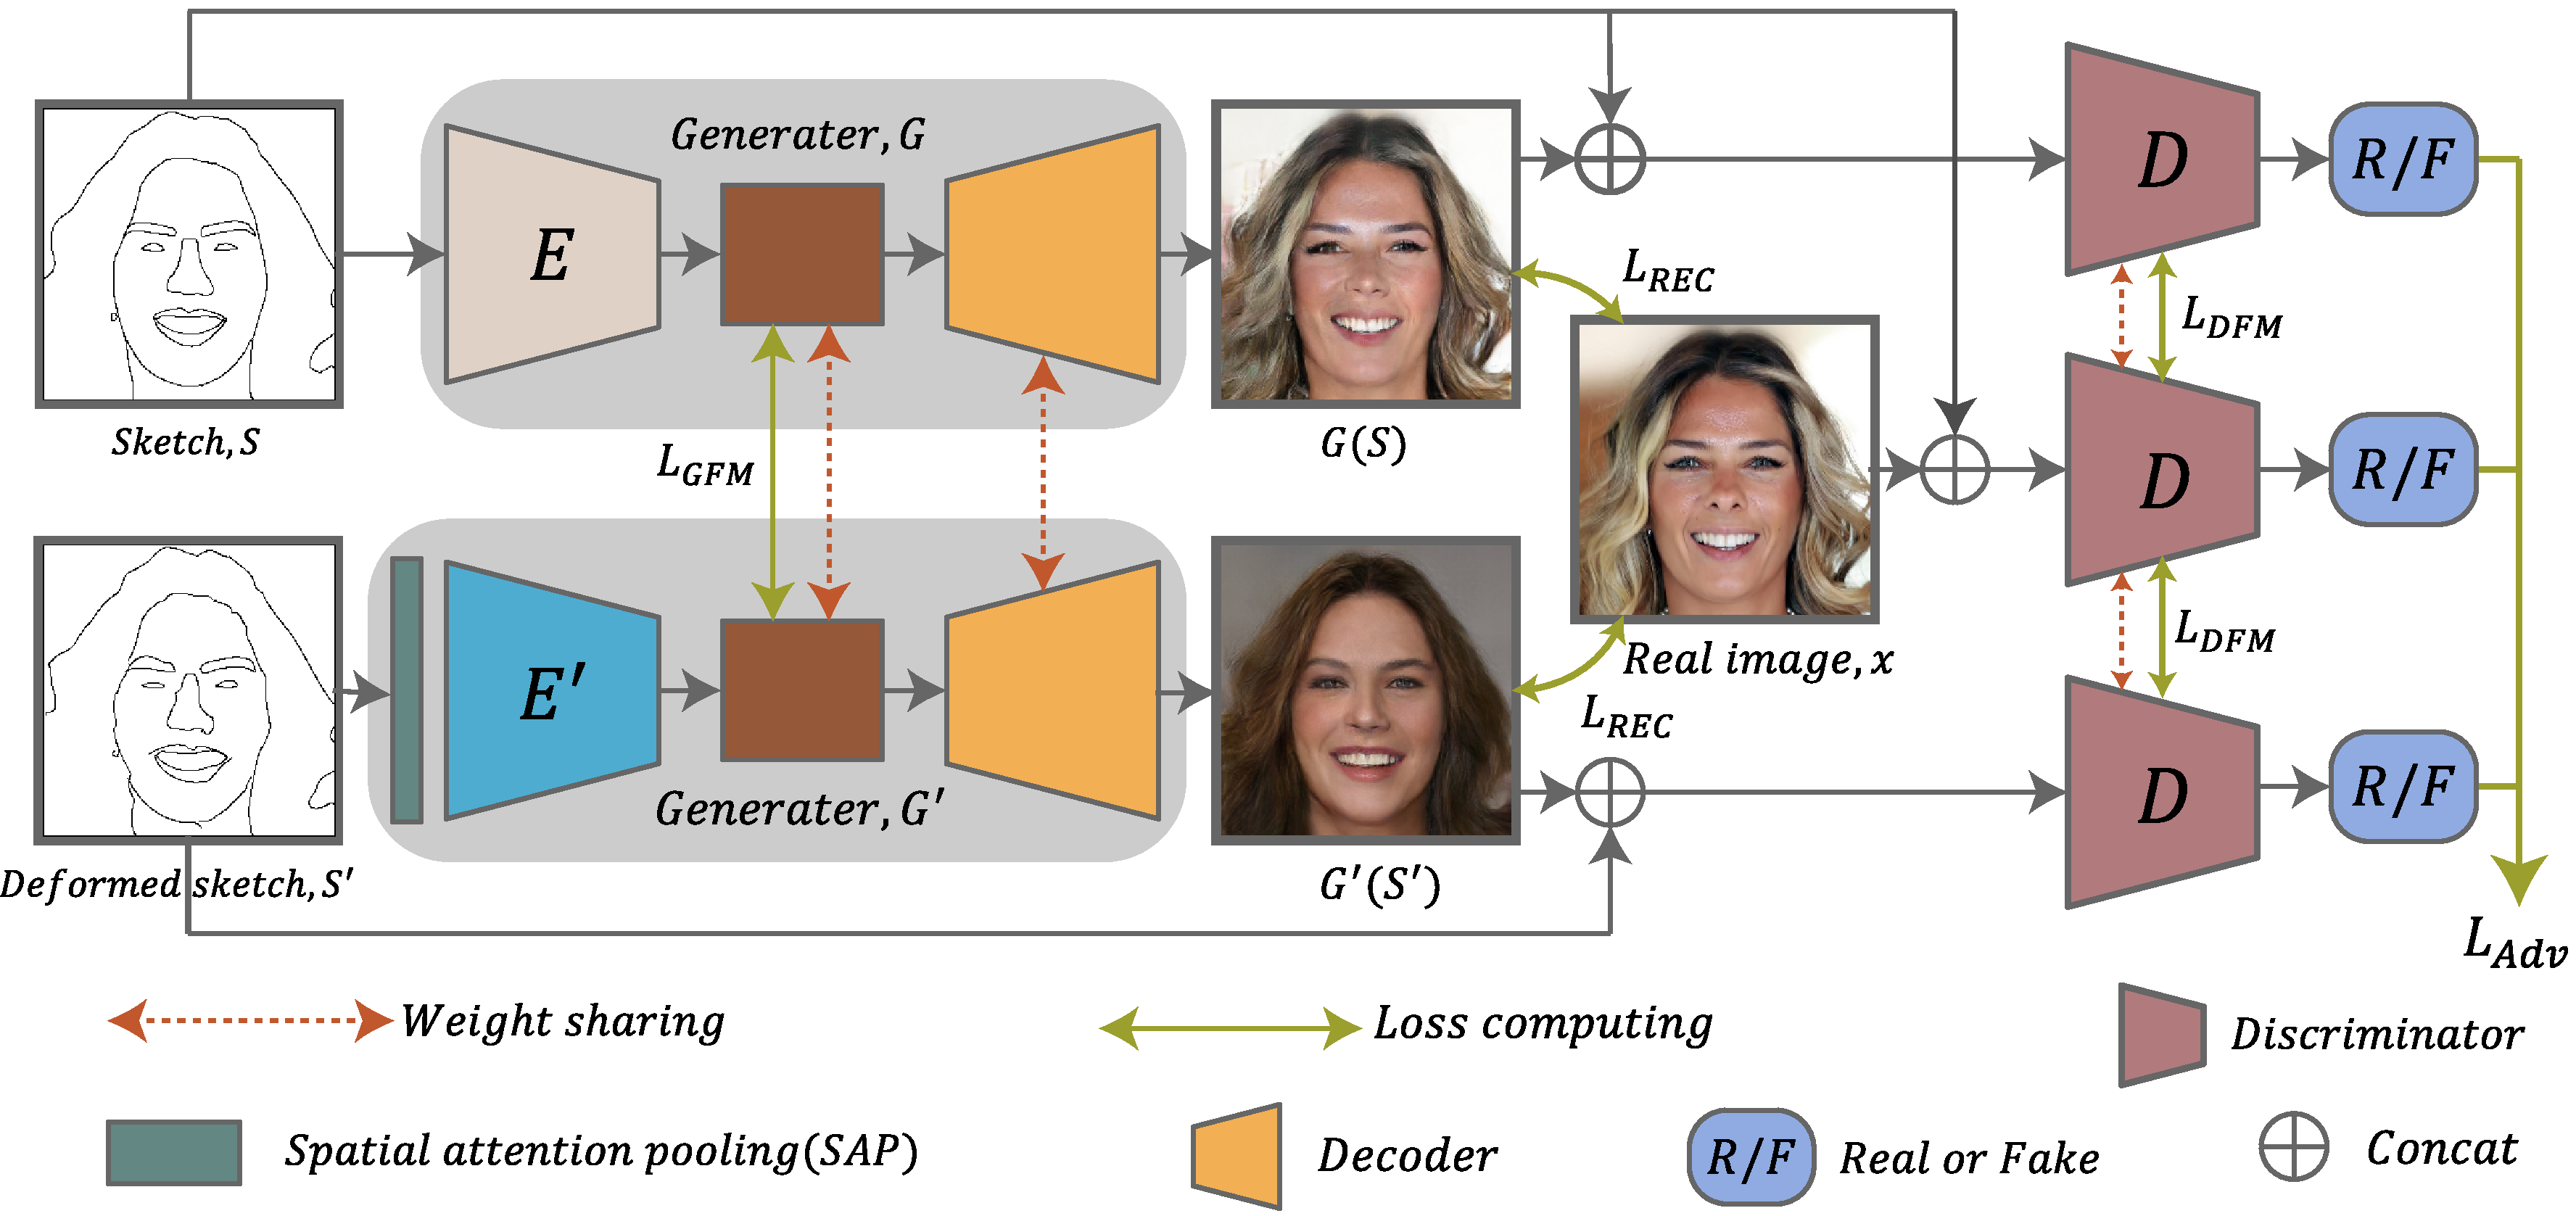
\includegraphics[width=\textwidth]{figs/architecture.png}
	\caption{The architecture of our model.}
	\label{fig:architecture}
\end{figure*}
%


%\subsection{Model Overview}
%\label{subsec:algorithm_overview}
Sketches drawn by users without well-trained drawing skills always contain severe line distortion, which may bring large degeneration to the generated face images and therefore damage the their quality hugely.
%
For this reason, we propose a sketch-to-photo translation model that is able to adaptively handle the line distortion of input sketches.

The architecture of the proposed model is shown in Figure~\ref{fig:architecture}. We use pix2pixHD model~\cite{pix2pixHD} with the 'global' version generator and the multi-scale discriminator with three sub-discriminators as the baseline model. The input of the generator is either a face sketch or a deformed face sketch and the output is the corresponding generated photo-realistic face image. A novel module named Spatial Attention Pooling (SAP) is added in the front of the generator to enable our model to adaptively handle line distortions of input sketches \td(before the lowest level of feature extraction.) 
%
For the discriminator, the generated image concatenated with the input sketch (or the deformed input sketch) is treated as a fake sample while a real face image sampled from real face distribution concatenated with its corresponding sketch is regarded as a real sample. 
%
%In the adversarial training stage, the generator and the discriminator are updated alternately.
%
In order to guided the model with SAP to be tolerant with line distortion of input sketches, we design a novel generator feature matching loss and an edge penalty \td{(a temporary name of this term)} for our task, besides the adversarial loss, the reconstruction loss and the discriminator feature matching loss used in pix2pixHD.
%

In this section, we first introduce the dataset we use in our experiment in Subsection~\ref{subsec:algorithm_}. Then we describe the proposed SAP in subsection~\ref{subsec:algorithm_sap}. At last we discuss losses we apply in Subsection~\ref{subsec:algorithm_loss}.

